\begin{tikzpicture}[scale=.2, anchor=west]
\node[draw opacity=0, fill opacity=0, anchor=south west] (dummyL) at (-3, -15){};
\node[draw=black, rectangle split, anchor=south west, rectangle split parts=3] (sn0x8671148) at ([xshift=2cm]dummyL){
\begin{tikzpicture}[scale=.2]
\node[circle, scale=0.75, fill] (tid0) at (3,1.5){};
\node[circle, scale=0.75, fill] (tid1) at (2.25,3){};
\node[circle, scale=0.75, fill] (tid3) at (1.5,4.5){};
\node[circle, scale=0.75, fill] (tid6) at (0.75,6){};
\node[circle, scale=0.75, fill] (tid9) at (0.75,7.5){};
\node[circle, scale=0.75, fill, red] (tid10) at (0.75,9){};
\draw[](tid9) -- (tid10);
\draw[](tid6) -- (tid9);
\node[circle, scale=0.75, fill, red] (tid7) at (2.25,6){};
\draw[](tid3) -- (tid6);
\draw[](tid3) -- (tid7);
\node[circle, scale=0.75, fill] (tid4) at (3.75,4.5){};
\node[circle, scale=0.75, fill, red] (tid8) at (3.75,6){};
\draw[](tid4) -- (tid8);
\draw[](tid1) -- (tid3);
\draw[](tid1) -- (tid4);
\node[circle, scale=0.75, fill] (tid2) at (5.25,3){};
\node[circle, scale=0.75, fill] (tid5) at (5.25,4.5){};
\draw[](tid2) -- (tid5);
\draw[](tid0) -- (tid1);
\draw[](tid0) -- (tid2);
\end{tikzpicture}
\nodepart{two}
\footnotesize{6.51697}
\nodepart{three}
\footnotesize{$33\:17\:17\:33$}
};
\node[draw opacity=0, fill opacity=0, anchor=south west] (dummyL) at (-12, -30){};
\node[draw=black, rectangle split, anchor=south west, rectangle split parts=3] (sn0x8673440) at ([xshift=2cm]dummyL){
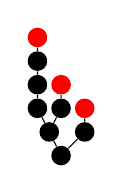
\begin{tikzpicture}[scale=.2]
\node[circle, scale=0.75, fill] (tid0) at (2.25,1.5){};
\node[circle, scale=0.75, fill] (tid1) at (1.5,3){};
\node[circle, scale=0.75, fill] (tid3) at (0.75,4.5){};
\node[circle, scale=0.75, fill] (tid6) at (0.75,6){};
\node[circle, scale=0.75, fill] (tid8) at (0.75,7.5){};
\node[circle, scale=0.75, fill, red] (tid9) at (0.75,9){};
\draw[](tid8) -- (tid9);
\draw[](tid6) -- (tid8);
\draw[](tid3) -- (tid6);
\node[circle, scale=0.75, fill] (tid4) at (2.25,4.5){};
\node[circle, scale=0.75, fill, red] (tid7) at (2.25,6){};
\draw[](tid4) -- (tid7);
\draw[](tid1) -- (tid3);
\draw[](tid1) -- (tid4);
\node[circle, scale=0.75, fill] (tid2) at (3.75,3){};
\node[circle, scale=0.75, fill, red] (tid5) at (3.75,4.5){};
\draw[](tid2) -- (tid5);
\draw[](tid0) -- (tid1);
\draw[](tid0) -- (tid2);
\end{tikzpicture}
\nodepart{two}
\footnotesize{6.35933}
\nodepart{three}
\footnotesize{$33\:33\:33$}
};
\node[draw opacity=0, fill opacity=0, anchor=south west] (dummyL) at (-12, -30){};
\node[draw=black, rectangle split, anchor=south west, rectangle split parts=3] (sn0x8672868) at ([xshift=2cm]sn0x8673440.south east){
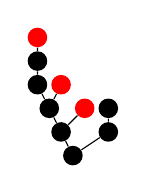
\begin{tikzpicture}[scale=.2]
\node[circle, scale=0.75, fill] (tid0) at (3,1.5){};
\node[circle, scale=0.75, fill] (tid1) at (2.25,3){};
\node[circle, scale=0.75, fill] (tid3) at (1.5,4.5){};
\node[circle, scale=0.75, fill] (tid6) at (0.75,6){};
\node[circle, scale=0.75, fill] (tid8) at (0.75,7.5){};
\node[circle, scale=0.75, fill, red] (tid9) at (0.75,9){};
\draw[](tid8) -- (tid9);
\draw[](tid6) -- (tid8);
\node[circle, scale=0.75, fill, red] (tid7) at (2.25,6){};
\draw[](tid3) -- (tid6);
\draw[](tid3) -- (tid7);
\node[circle, scale=0.75, fill, red] (tid4) at (3.75,4.5){};
\draw[](tid1) -- (tid3);
\draw[](tid1) -- (tid4);
\node[circle, scale=0.75, fill] (tid2) at (5.25,3){};
\node[circle, scale=0.75, fill] (tid5) at (5.25,4.5){};
\draw[](tid2) -- (tid5);
\draw[](tid0) -- (tid1);
\draw[](tid0) -- (tid2);
\end{tikzpicture}
\nodepart{two}
\footnotesize{6.34949}
\nodepart{three}
\footnotesize{$33\:33\:33$}
};
\node[draw opacity=0, fill opacity=0, anchor=south west] (dummyL) at (-12, -30){};
\node[draw=black, rectangle split, anchor=south west, rectangle split parts=3] (sn0x86715f8) at ([xshift=2cm]sn0x8672868.south east){
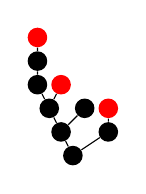
\begin{tikzpicture}[scale=.2]
\node[circle, scale=0.75, fill] (tid0) at (3,1.5){};
\node[circle, scale=0.75, fill] (tid1) at (2.25,3){};
\node[circle, scale=0.75, fill] (tid3) at (1.5,4.5){};
\node[circle, scale=0.75, fill] (tid6) at (0.75,6){};
\node[circle, scale=0.75, fill] (tid8) at (0.75,7.5){};
\node[circle, scale=0.75, fill, red] (tid9) at (0.75,9){};
\draw[](tid8) -- (tid9);
\draw[](tid6) -- (tid8);
\node[circle, scale=0.75, fill, red] (tid7) at (2.25,6){};
\draw[](tid3) -- (tid6);
\draw[](tid3) -- (tid7);
\node[circle, scale=0.75, fill] (tid4) at (3.75,4.5){};
\draw[](tid1) -- (tid3);
\draw[](tid1) -- (tid4);
\node[circle, scale=0.75, fill] (tid2) at (5.25,3){};
\node[circle, scale=0.75, fill, red] (tid5) at (5.25,4.5){};
\draw[](tid2) -- (tid5);
\draw[](tid0) -- (tid1);
\draw[](tid0) -- (tid2);
\end{tikzpicture}
\nodepart{two}
\footnotesize{6.33194}
\nodepart{three}
\footnotesize{$33\:33\:33$}
};
\node[draw opacity=0, fill opacity=0, anchor=south west] (dummyL) at (-12, -30){};
\node[draw=black, rectangle split, anchor=south west, rectangle split parts=3] (sn0x8671730) at ([xshift=2cm]sn0x86715f8.south east){
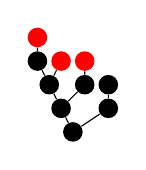
\begin{tikzpicture}[scale=.2]
\node[circle, scale=0.75, fill] (tid0) at (3,1.5){};
\node[circle, scale=0.75, fill] (tid1) at (2.25,3){};
\node[circle, scale=0.75, fill] (tid3) at (1.5,4.5){};
\node[circle, scale=0.75, fill] (tid6) at (0.75,6){};
\node[circle, scale=0.75, fill, red] (tid9) at (0.75,7.5){};
\draw[](tid6) -- (tid9);
\node[circle, scale=0.75, fill, red] (tid7) at (2.25,6){};
\draw[](tid3) -- (tid6);
\draw[](tid3) -- (tid7);
\node[circle, scale=0.75, fill] (tid4) at (3.75,4.5){};
\node[circle, scale=0.75, fill, red] (tid8) at (3.75,6){};
\draw[](tid4) -- (tid8);
\draw[](tid1) -- (tid3);
\draw[](tid1) -- (tid4);
\node[circle, scale=0.75, fill] (tid2) at (5.25,3){};
\node[circle, scale=0.75, fill] (tid5) at (5.25,4.5){};
\draw[](tid2) -- (tid5);
\draw[](tid0) -- (tid1);
\draw[](tid0) -- (tid2);
\end{tikzpicture}
\nodepart{two}
\footnotesize{5.85087}
\nodepart{three}
\footnotesize{$33\:17\:17\:33$}
};
\node[draw opacity=0, fill opacity=0, anchor=south west] (dummyL) at (-24, -45){};
\node[draw=black, rectangle split, anchor=south west, rectangle split parts=3] (sn0x8674070) at ([xshift=2cm]dummyL){
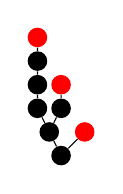
\begin{tikzpicture}[scale=.2]
\node[circle, scale=0.75, fill] (tid0) at (2.25,1.5){};
\node[circle, scale=0.75, fill] (tid1) at (1.5,3){};
\node[circle, scale=0.75, fill] (tid3) at (0.75,4.5){};
\node[circle, scale=0.75, fill] (tid5) at (0.75,6){};
\node[circle, scale=0.75, fill] (tid7) at (0.75,7.5){};
\node[circle, scale=0.75, fill, red] (tid8) at (0.75,9){};
\draw[](tid7) -- (tid8);
\draw[](tid5) -- (tid7);
\draw[](tid3) -- (tid5);
\node[circle, scale=0.75, fill] (tid4) at (2.25,4.5){};
\node[circle, scale=0.75, fill, red] (tid6) at (2.25,6){};
\draw[](tid4) -- (tid6);
\draw[](tid1) -- (tid3);
\draw[](tid1) -- (tid4);
\node[circle, scale=0.75, fill, red] (tid2) at (3.75,3){};
\draw[](tid0) -- (tid1);
\draw[](tid0) -- (tid2);
\end{tikzpicture}
\nodepart{two}
\footnotesize{6.27251}
\nodepart{three}
\footnotesize{$33\:33\:33$}
};
\node[draw opacity=0, fill opacity=0, anchor=south west] (dummyL) at (-24, -45){};
\node[draw=black, rectangle split, anchor=south west, rectangle split parts=3] (sn0x8670960) at ([xshift=2cm]sn0x8674070.south east){
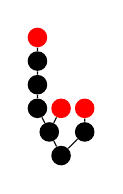
\begin{tikzpicture}[scale=.2]
\node[circle, scale=0.75, fill] (tid0) at (2.25,1.5){};
\node[circle, scale=0.75, fill] (tid1) at (1.5,3){};
\node[circle, scale=0.75, fill] (tid3) at (0.75,4.5){};
\node[circle, scale=0.75, fill] (tid6) at (0.75,6){};
\node[circle, scale=0.75, fill] (tid7) at (0.75,7.5){};
\node[circle, scale=0.75, fill, red] (tid8) at (0.75,9){};
\draw[](tid7) -- (tid8);
\draw[](tid6) -- (tid7);
\draw[](tid3) -- (tid6);
\node[circle, scale=0.75, fill, red] (tid4) at (2.25,4.5){};
\draw[](tid1) -- (tid3);
\draw[](tid1) -- (tid4);
\node[circle, scale=0.75, fill] (tid2) at (3.75,3){};
\node[circle, scale=0.75, fill, red] (tid5) at (3.75,4.5){};
\draw[](tid2) -- (tid5);
\draw[](tid0) -- (tid1);
\draw[](tid0) -- (tid2);
\end{tikzpicture}
\nodepart{two}
\footnotesize{6.19284}
\nodepart{three}
\footnotesize{$33\:33\:33$}
};
\node[draw opacity=0, fill opacity=0, anchor=south west] (dummyL) at (-24, -45){};
\node[draw=black, rectangle split, anchor=south west, rectangle split parts=3] (sn0x8671f38) at ([xshift=2cm]sn0x8670960.south east){
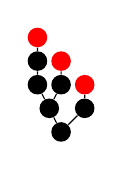
\begin{tikzpicture}[scale=.2]
\node[circle, scale=0.75, fill] (tid0) at (2.25,1.5){};
\node[circle, scale=0.75, fill] (tid1) at (1.5,3){};
\node[circle, scale=0.75, fill] (tid3) at (0.75,4.5){};
\node[circle, scale=0.75, fill] (tid6) at (0.75,6){};
\node[circle, scale=0.75, fill, red] (tid8) at (0.75,7.5){};
\draw[](tid6) -- (tid8);
\draw[](tid3) -- (tid6);
\node[circle, scale=0.75, fill] (tid4) at (2.25,4.5){};
\node[circle, scale=0.75, fill, red] (tid7) at (2.25,6){};
\draw[](tid4) -- (tid7);
\draw[](tid1) -- (tid3);
\draw[](tid1) -- (tid4);
\node[circle, scale=0.75, fill] (tid2) at (3.75,3){};
\node[circle, scale=0.75, fill, red] (tid5) at (3.75,4.5){};
\draw[](tid2) -- (tid5);
\draw[](tid0) -- (tid1);
\draw[](tid0) -- (tid2);
\end{tikzpicture}
\nodepart{two}
\footnotesize{5.61266}
\nodepart{three}
\footnotesize{$33\:33\:33$}
};
\node[draw opacity=0, fill opacity=0, anchor=south west] (dummyL) at (-24, -45){};
\node[draw=black, rectangle split, anchor=south west, rectangle split parts=3] (sn0x8679150) at ([xshift=2cm]sn0x8671f38.south east){
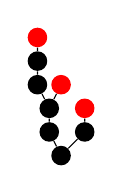
\begin{tikzpicture}[scale=.2]
\node[circle, scale=0.75, fill] (tid0) at (2.25,1.5){};
\node[circle, scale=0.75, fill] (tid1) at (1.5,3){};
\node[circle, scale=0.75, fill] (tid3) at (1.5,4.5){};
\node[circle, scale=0.75, fill] (tid5) at (0.75,6){};
\node[circle, scale=0.75, fill] (tid7) at (0.75,7.5){};
\node[circle, scale=0.75, fill, red] (tid8) at (0.75,9){};
\draw[](tid7) -- (tid8);
\draw[](tid5) -- (tid7);
\node[circle, scale=0.75, fill, red] (tid6) at (2.25,6){};
\draw[](tid3) -- (tid5);
\draw[](tid3) -- (tid6);
\draw[](tid1) -- (tid3);
\node[circle, scale=0.75, fill] (tid2) at (3.75,3){};
\node[circle, scale=0.75, fill, red] (tid4) at (3.75,4.5){};
\draw[](tid2) -- (tid4);
\draw[](tid0) -- (tid1);
\draw[](tid0) -- (tid2);
\end{tikzpicture}
\nodepart{two}
\footnotesize{6.24942}
\nodepart{three}
\footnotesize{$33\:33\:33$}
};
\node[draw opacity=0, fill opacity=0, anchor=south west] (dummyL) at (-24, -45){};
\node[draw=black, rectangle split, anchor=south west, rectangle split parts=3] (sn0x8678838) at ([xshift=2cm]sn0x8679150.south east){
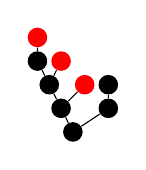
\begin{tikzpicture}[scale=.2]
\node[circle, scale=0.75, fill] (tid0) at (3,1.5){};
\node[circle, scale=0.75, fill] (tid1) at (2.25,3){};
\node[circle, scale=0.75, fill] (tid3) at (1.5,4.5){};
\node[circle, scale=0.75, fill] (tid6) at (0.75,6){};
\node[circle, scale=0.75, fill, red] (tid8) at (0.75,7.5){};
\draw[](tid6) -- (tid8);
\node[circle, scale=0.75, fill, red] (tid7) at (2.25,6){};
\draw[](tid3) -- (tid6);
\draw[](tid3) -- (tid7);
\node[circle, scale=0.75, fill, red] (tid4) at (3.75,4.5){};
\draw[](tid1) -- (tid3);
\draw[](tid1) -- (tid4);
\node[circle, scale=0.75, fill] (tid2) at (5.25,3){};
\node[circle, scale=0.75, fill] (tid5) at (5.25,4.5){};
\draw[](tid2) -- (tid5);
\draw[](tid0) -- (tid1);
\draw[](tid0) -- (tid2);
\end{tikzpicture}
\nodepart{two}
\footnotesize{5.60623}
\nodepart{three}
\footnotesize{$33\:33\:33$}
};
\node[draw opacity=0, fill opacity=0, anchor=south west] (dummyL) at (-24, -45){};
\node[draw=black, rectangle split, anchor=south west, rectangle split parts=3] (sn0x867b748) at ([xshift=2cm]sn0x8678838.south east){
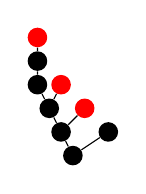
\begin{tikzpicture}[scale=.2]
\node[circle, scale=0.75, fill] (tid0) at (3,1.5){};
\node[circle, scale=0.75, fill] (tid1) at (2.25,3){};
\node[circle, scale=0.75, fill] (tid3) at (1.5,4.5){};
\node[circle, scale=0.75, fill] (tid5) at (0.75,6){};
\node[circle, scale=0.75, fill] (tid7) at (0.75,7.5){};
\node[circle, scale=0.75, fill, red] (tid8) at (0.75,9){};
\draw[](tid7) -- (tid8);
\draw[](tid5) -- (tid7);
\node[circle, scale=0.75, fill, red] (tid6) at (2.25,6){};
\draw[](tid3) -- (tid5);
\draw[](tid3) -- (tid6);
\node[circle, scale=0.75, fill, red] (tid4) at (3.75,4.5){};
\draw[](tid1) -- (tid3);
\draw[](tid1) -- (tid4);
\node[circle, scale=0.75, fill] (tid2) at (5.25,3){};
\draw[](tid0) -- (tid1);
\draw[](tid0) -- (tid2);
\end{tikzpicture}
\nodepart{two}
\footnotesize{6.21811}
\nodepart{three}
\footnotesize{$33\:33\:33$}
};
\node[draw opacity=0, fill opacity=0, anchor=south west] (dummyL) at (-24, -45){};
\node[draw=black, rectangle split, anchor=south west, rectangle split parts=3] (sn0x867b6e8) at ([xshift=2cm]sn0x867b748.south east){
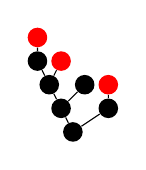
\begin{tikzpicture}[scale=.2]
\node[circle, scale=0.75, fill] (tid0) at (3,1.5){};
\node[circle, scale=0.75, fill] (tid1) at (2.25,3){};
\node[circle, scale=0.75, fill] (tid3) at (1.5,4.5){};
\node[circle, scale=0.75, fill] (tid6) at (0.75,6){};
\node[circle, scale=0.75, fill, red] (tid8) at (0.75,7.5){};
\draw[](tid6) -- (tid8);
\node[circle, scale=0.75, fill, red] (tid7) at (2.25,6){};
\draw[](tid3) -- (tid6);
\draw[](tid3) -- (tid7);
\node[circle, scale=0.75, fill] (tid4) at (3.75,4.5){};
\draw[](tid1) -- (tid3);
\draw[](tid1) -- (tid4);
\node[circle, scale=0.75, fill] (tid2) at (5.25,3){};
\node[circle, scale=0.75, fill, red] (tid5) at (5.25,4.5){};
\draw[](tid2) -- (tid5);
\draw[](tid0) -- (tid1);
\draw[](tid0) -- (tid2);
\end{tikzpicture}
\nodepart{two}
\footnotesize{5.58488}
\nodepart{three}
\footnotesize{$33\:33\:33$}
};
\node[draw opacity=0, fill opacity=0, anchor=south west] (dummyL) at (-24, -45){};
\node[draw=black, rectangle split, anchor=south west, rectangle split parts=3] (sn0x867c970) at ([xshift=2cm]sn0x867b6e8.south east){
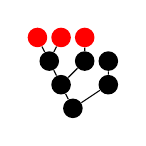
\begin{tikzpicture}[scale=.2]
\node[circle, scale=0.75, fill] (tid0) at (3,1.5){};
\node[circle, scale=0.75, fill] (tid1) at (2.25,3){};
\node[circle, scale=0.75, fill] (tid3) at (1.5,4.5){};
\node[circle, scale=0.75, fill, red] (tid6) at (0.75,6){};
\node[circle, scale=0.75, fill, red] (tid7) at (2.25,6){};
\draw[](tid3) -- (tid6);
\draw[](tid3) -- (tid7);
\node[circle, scale=0.75, fill] (tid4) at (3.75,4.5){};
\node[circle, scale=0.75, fill, red] (tid8) at (3.75,6){};
\draw[](tid4) -- (tid8);
\draw[](tid1) -- (tid3);
\draw[](tid1) -- (tid4);
\node[circle, scale=0.75, fill] (tid2) at (5.25,3){};
\node[circle, scale=0.75, fill] (tid5) at (5.25,4.5){};
\draw[](tid2) -- (tid5);
\draw[](tid0) -- (tid1);
\draw[](tid0) -- (tid2);
\end{tikzpicture}
\nodepart{two}
\footnotesize{5.34439}
\nodepart{three}
\footnotesize{$67\:17\:17$}
};
\node[draw opacity=0, fill opacity=0, anchor=south west] (dummyL) at (-33, -60){};
\node[draw=black, rectangle split, anchor=south west, rectangle split parts=3] (sn0x86717a8) at ([xshift=2cm]dummyL){
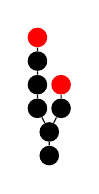
\begin{tikzpicture}[scale=.2]
\node[circle, scale=0.75, fill] (tid0) at (1.5,1.5){};
\node[circle, scale=0.75, fill] (tid1) at (1.5,3){};
\node[circle, scale=0.75, fill] (tid2) at (0.75,4.5){};
\node[circle, scale=0.75, fill] (tid4) at (0.75,6){};
\node[circle, scale=0.75, fill] (tid6) at (0.75,7.5){};
\node[circle, scale=0.75, fill, red] (tid7) at (0.75,9){};
\draw[](tid6) -- (tid7);
\draw[](tid4) -- (tid6);
\draw[](tid2) -- (tid4);
\node[circle, scale=0.75, fill] (tid3) at (2.25,4.5){};
\node[circle, scale=0.75, fill, red] (tid5) at (2.25,6){};
\draw[](tid3) -- (tid5);
\draw[](tid1) -- (tid2);
\draw[](tid1) -- (tid3);
\draw[](tid0) -- (tid1);
\end{tikzpicture}
\nodepart{two}
\footnotesize{6.25}
\nodepart{three}
\footnotesize{$50\:50$}
};
\node[draw opacity=0, fill opacity=0, anchor=south west] (dummyL) at (-33, -60){};
\node[draw=black, rectangle split, anchor=south west, rectangle split parts=3] (sn0x8674958) at ([xshift=2cm]sn0x86717a8.south east){
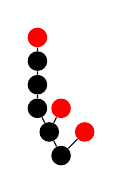
\begin{tikzpicture}[scale=.2]
\node[circle, scale=0.75, fill] (tid0) at (2.25,1.5){};
\node[circle, scale=0.75, fill] (tid1) at (1.5,3){};
\node[circle, scale=0.75, fill] (tid3) at (0.75,4.5){};
\node[circle, scale=0.75, fill] (tid5) at (0.75,6){};
\node[circle, scale=0.75, fill] (tid6) at (0.75,7.5){};
\node[circle, scale=0.75, fill, red] (tid7) at (0.75,9){};
\draw[](tid6) -- (tid7);
\draw[](tid5) -- (tid6);
\draw[](tid3) -- (tid5);
\node[circle, scale=0.75, fill, red] (tid4) at (2.25,4.5){};
\draw[](tid1) -- (tid3);
\draw[](tid1) -- (tid4);
\node[circle, scale=0.75, fill, red] (tid2) at (3.75,3){};
\draw[](tid0) -- (tid1);
\draw[](tid0) -- (tid2);
\end{tikzpicture}
\nodepart{two}
\footnotesize{6.09066}
\nodepart{three}
\footnotesize{$33\:33\:33$}
};
\node[draw opacity=0, fill opacity=0, anchor=south west] (dummyL) at (-33, -60){};
\node[draw=black, rectangle split, anchor=south west, rectangle split parts=3] (sn0x8674cb0) at ([xshift=2cm]sn0x8674958.south east){
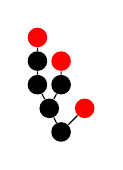
\begin{tikzpicture}[scale=.2]
\node[circle, scale=0.75, fill] (tid0) at (2.25,1.5){};
\node[circle, scale=0.75, fill] (tid1) at (1.5,3){};
\node[circle, scale=0.75, fill] (tid3) at (0.75,4.5){};
\node[circle, scale=0.75, fill] (tid5) at (0.75,6){};
\node[circle, scale=0.75, fill, red] (tid7) at (0.75,7.5){};
\draw[](tid5) -- (tid7);
\draw[](tid3) -- (tid5);
\node[circle, scale=0.75, fill] (tid4) at (2.25,4.5){};
\node[circle, scale=0.75, fill, red] (tid6) at (2.25,6){};
\draw[](tid4) -- (tid6);
\draw[](tid1) -- (tid3);
\draw[](tid1) -- (tid4);
\node[circle, scale=0.75, fill, red] (tid2) at (3.75,3){};
\draw[](tid0) -- (tid1);
\draw[](tid0) -- (tid2);
\end{tikzpicture}
\nodepart{two}
\footnotesize{5.47685}
\nodepart{three}
\footnotesize{$33\:33\:33$}
};
\node[draw opacity=0, fill opacity=0, anchor=south west] (dummyL) at (-33, -60){};
\node[draw=black, rectangle split, anchor=south west, rectangle split parts=3] (sn0x8677a00) at ([xshift=2cm]sn0x8674cb0.south east){
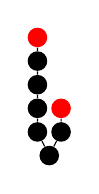
\begin{tikzpicture}[scale=.2]
\node[circle, scale=0.75, fill] (tid0) at (1.5,1.5){};
\node[circle, scale=0.75, fill] (tid1) at (0.75,3){};
\node[circle, scale=0.75, fill] (tid3) at (0.75,4.5){};
\node[circle, scale=0.75, fill] (tid5) at (0.75,6){};
\node[circle, scale=0.75, fill] (tid6) at (0.75,7.5){};
\node[circle, scale=0.75, fill, red] (tid7) at (0.75,9){};
\draw[](tid6) -- (tid7);
\draw[](tid5) -- (tid6);
\draw[](tid3) -- (tid5);
\draw[](tid1) -- (tid3);
\node[circle, scale=0.75, fill] (tid2) at (2.25,3){};
\node[circle, scale=0.75, fill, red] (tid4) at (2.25,4.5){};
\draw[](tid2) -- (tid4);
\draw[](tid0) -- (tid1);
\draw[](tid0) -- (tid2);
\end{tikzpicture}
\nodepart{two}
\footnotesize{6.14062}
\nodepart{three}
\footnotesize{$50\:50$}
};
\node[draw opacity=0, fill opacity=0, anchor=south west] (dummyL) at (-33, -60){};
\node[draw=black, rectangle split, anchor=south west, rectangle split parts=3] (sn0x8677b20) at ([xshift=2cm]sn0x8677a00.south east){
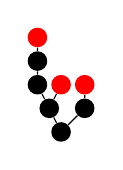
\begin{tikzpicture}[scale=.2]
\node[circle, scale=0.75, fill] (tid0) at (2.25,1.5){};
\node[circle, scale=0.75, fill] (tid1) at (1.5,3){};
\node[circle, scale=0.75, fill] (tid3) at (0.75,4.5){};
\node[circle, scale=0.75, fill] (tid6) at (0.75,6){};
\node[circle, scale=0.75, fill, red] (tid7) at (0.75,7.5){};
\draw[](tid6) -- (tid7);
\draw[](tid3) -- (tid6);
\node[circle, scale=0.75, fill, red] (tid4) at (2.25,4.5){};
\draw[](tid1) -- (tid3);
\draw[](tid1) -- (tid4);
\node[circle, scale=0.75, fill] (tid2) at (3.75,3){};
\node[circle, scale=0.75, fill, red] (tid5) at (3.75,4.5){};
\draw[](tid2) -- (tid5);
\draw[](tid0) -- (tid1);
\draw[](tid0) -- (tid2);
\end{tikzpicture}
\nodepart{two}
\footnotesize{5.34722}
\nodepart{three}
\footnotesize{$33\:33\:33$}
};
\node[draw opacity=0, fill opacity=0, anchor=south west] (dummyL) at (-33, -60){};
\node[draw=black, rectangle split, anchor=south west, rectangle split parts=3] (sn0x86791a8) at ([xshift=2cm]sn0x8677b20.south east){
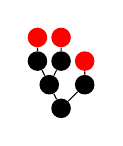
\begin{tikzpicture}[scale=.2]
\node[circle, scale=0.75, fill] (tid0) at (2.25,1.5){};
\node[circle, scale=0.75, fill] (tid1) at (1.5,3){};
\node[circle, scale=0.75, fill] (tid3) at (0.75,4.5){};
\node[circle, scale=0.75, fill, red] (tid6) at (0.75,6){};
\draw[](tid3) -- (tid6);
\node[circle, scale=0.75, fill] (tid4) at (2.25,4.5){};
\node[circle, scale=0.75, fill, red] (tid7) at (2.25,6){};
\draw[](tid4) -- (tid7);
\draw[](tid1) -- (tid3);
\draw[](tid1) -- (tid4);
\node[circle, scale=0.75, fill] (tid2) at (3.75,3){};
\node[circle, scale=0.75, fill, red] (tid5) at (3.75,4.5){};
\draw[](tid2) -- (tid5);
\draw[](tid0) -- (tid1);
\draw[](tid0) -- (tid2);
\end{tikzpicture}
\nodepart{two}
\footnotesize{5.01389}
\nodepart{three}
\footnotesize{$33\:67$}
};
\node[draw opacity=0, fill opacity=0, anchor=south west] (dummyL) at (-33, -60){};
\node[draw=black, rectangle split, anchor=south west, rectangle split parts=3] (sn0x8679ac0) at ([xshift=2cm]sn0x86791a8.south east){
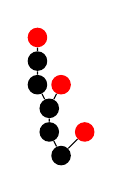
\begin{tikzpicture}[scale=.2]
\node[circle, scale=0.75, fill] (tid0) at (2.25,1.5){};
\node[circle, scale=0.75, fill] (tid1) at (1.5,3){};
\node[circle, scale=0.75, fill] (tid3) at (1.5,4.5){};
\node[circle, scale=0.75, fill] (tid4) at (0.75,6){};
\node[circle, scale=0.75, fill] (tid6) at (0.75,7.5){};
\node[circle, scale=0.75, fill, red] (tid7) at (0.75,9){};
\draw[](tid6) -- (tid7);
\draw[](tid4) -- (tid6);
\node[circle, scale=0.75, fill, red] (tid5) at (2.25,6){};
\draw[](tid3) -- (tid4);
\draw[](tid3) -- (tid5);
\draw[](tid1) -- (tid3);
\node[circle, scale=0.75, fill, red] (tid2) at (3.75,3){};
\draw[](tid0) -- (tid1);
\draw[](tid0) -- (tid2);
\end{tikzpicture}
\nodepart{two}
\footnotesize{6.15162}
\nodepart{three}
\footnotesize{$33\:33\:33$}
};
\node[draw opacity=0, fill opacity=0, anchor=south west] (dummyL) at (-33, -60){};
\node[draw=black, rectangle split, anchor=south west, rectangle split parts=3] (sn0x8679030) at ([xshift=2cm]sn0x8679ac0.south east){
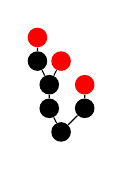
\begin{tikzpicture}[scale=.2]
\node[circle, scale=0.75, fill] (tid0) at (2.25,1.5){};
\node[circle, scale=0.75, fill] (tid1) at (1.5,3){};
\node[circle, scale=0.75, fill] (tid3) at (1.5,4.5){};
\node[circle, scale=0.75, fill] (tid5) at (0.75,6){};
\node[circle, scale=0.75, fill, red] (tid7) at (0.75,7.5){};
\draw[](tid5) -- (tid7);
\node[circle, scale=0.75, fill, red] (tid6) at (2.25,6){};
\draw[](tid3) -- (tid5);
\draw[](tid3) -- (tid6);
\draw[](tid1) -- (tid3);
\node[circle, scale=0.75, fill] (tid2) at (3.75,3){};
\node[circle, scale=0.75, fill, red] (tid4) at (3.75,4.5){};
\draw[](tid2) -- (tid4);
\draw[](tid0) -- (tid1);
\draw[](tid0) -- (tid2);
\end{tikzpicture}
\nodepart{two}
\footnotesize{5.45602}
\nodepart{three}
\footnotesize{$33\:33\:33$}
};
\node[draw opacity=0, fill opacity=0, anchor=south west] (dummyL) at (-33, -60){};
\node[draw=black, rectangle split, anchor=south west, rectangle split parts=3] (sn0x867b2e0) at ([xshift=2cm]sn0x8679030.south east){
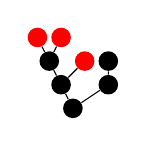
\begin{tikzpicture}[scale=.2]
\node[circle, scale=0.75, fill] (tid0) at (3,1.5){};
\node[circle, scale=0.75, fill] (tid1) at (2.25,3){};
\node[circle, scale=0.75, fill] (tid3) at (1.5,4.5){};
\node[circle, scale=0.75, fill, red] (tid6) at (0.75,6){};
\node[circle, scale=0.75, fill, red] (tid7) at (2.25,6){};
\draw[](tid3) -- (tid6);
\draw[](tid3) -- (tid7);
\node[circle, scale=0.75, fill, red] (tid4) at (3.75,4.5){};
\draw[](tid1) -- (tid3);
\draw[](tid1) -- (tid4);
\node[circle, scale=0.75, fill] (tid2) at (5.25,3){};
\node[circle, scale=0.75, fill] (tid5) at (5.25,4.5){};
\draw[](tid2) -- (tid5);
\draw[](tid0) -- (tid1);
\draw[](tid0) -- (tid2);
\end{tikzpicture}
\nodepart{two}
\footnotesize{5.01543}
\nodepart{three}
\footnotesize{$67\:33$}
};
\node[draw opacity=0, fill opacity=0, anchor=south west] (dummyL) at (-33, -60){};
\node[draw=black, rectangle split, anchor=south west, rectangle split parts=3] (sn0x867a9c8) at ([xshift=2cm]sn0x867b2e0.south east){
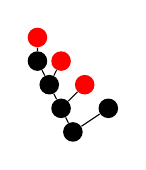
\begin{tikzpicture}[scale=.2]
\node[circle, scale=0.75, fill] (tid0) at (3,1.5){};
\node[circle, scale=0.75, fill] (tid1) at (2.25,3){};
\node[circle, scale=0.75, fill] (tid3) at (1.5,4.5){};
\node[circle, scale=0.75, fill] (tid5) at (0.75,6){};
\node[circle, scale=0.75, fill, red] (tid7) at (0.75,7.5){};
\draw[](tid5) -- (tid7);
\node[circle, scale=0.75, fill, red] (tid6) at (2.25,6){};
\draw[](tid3) -- (tid5);
\draw[](tid3) -- (tid6);
\node[circle, scale=0.75, fill, red] (tid4) at (3.75,4.5){};
\draw[](tid1) -- (tid3);
\draw[](tid1) -- (tid4);
\node[circle, scale=0.75, fill] (tid2) at (5.25,3){};
\draw[](tid0) -- (tid1);
\draw[](tid0) -- (tid2);
\end{tikzpicture}
\nodepart{two}
\footnotesize{5.41204}
\nodepart{three}
\footnotesize{$33\:33\:33$}
};
\node[draw opacity=0, fill opacity=0, anchor=south west] (dummyL) at (-33, -60){};
\node[draw=black, rectangle split, anchor=south west, rectangle split parts=3] (sn0x867b7c8) at ([xshift=2cm]sn0x867a9c8.south east){
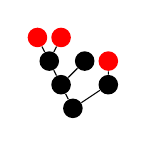
\begin{tikzpicture}[scale=.2]
\node[circle, scale=0.75, fill] (tid0) at (3,1.5){};
\node[circle, scale=0.75, fill] (tid1) at (2.25,3){};
\node[circle, scale=0.75, fill] (tid3) at (1.5,4.5){};
\node[circle, scale=0.75, fill, red] (tid6) at (0.75,6){};
\node[circle, scale=0.75, fill, red] (tid7) at (2.25,6){};
\draw[](tid3) -- (tid6);
\draw[](tid3) -- (tid7);
\node[circle, scale=0.75, fill] (tid4) at (3.75,4.5){};
\draw[](tid1) -- (tid3);
\draw[](tid1) -- (tid4);
\node[circle, scale=0.75, fill] (tid2) at (5.25,3){};
\node[circle, scale=0.75, fill, red] (tid5) at (5.25,4.5){};
\draw[](tid2) -- (tid5);
\draw[](tid0) -- (tid1);
\draw[](tid0) -- (tid2);
\end{tikzpicture}
\nodepart{two}
\footnotesize{4.99537}
\nodepart{three}
\footnotesize{$67\:33$}
};
\node[draw opacity=0, fill opacity=0, anchor=south west] (dummyL) at (-33, -75){};
\node[draw=black, rectangle split, anchor=south west, rectangle split parts=3] (sn0x8671678) at ([xshift=2cm]dummyL){
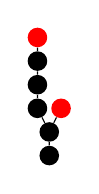
\begin{tikzpicture}[scale=.2]
\node[circle, scale=0.75, fill] (tid0) at (1.5,1.5){};
\node[circle, scale=0.75, fill] (tid1) at (1.5,3){};
\node[circle, scale=0.75, fill] (tid2) at (0.75,4.5){};
\node[circle, scale=0.75, fill] (tid4) at (0.75,6){};
\node[circle, scale=0.75, fill] (tid5) at (0.75,7.5){};
\node[circle, scale=0.75, fill, red] (tid6) at (0.75,9){};
\draw[](tid5) -- (tid6);
\draw[](tid4) -- (tid5);
\draw[](tid2) -- (tid4);
\node[circle, scale=0.75, fill, red] (tid3) at (2.25,4.5){};
\draw[](tid1) -- (tid2);
\draw[](tid1) -- (tid3);
\draw[](tid0) -- (tid1);
\end{tikzpicture}
\nodepart{two}
\footnotesize{6.0625}
\nodepart{three}
\footnotesize{$50\:50$}
};
\node[draw opacity=0, fill opacity=0, anchor=south west] (dummyL) at (-33, -75){};
\node[draw=black, rectangle split, anchor=south west, rectangle split parts=3] (sn0x8674888) at ([xshift=2cm]sn0x8671678.south east){
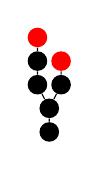
\begin{tikzpicture}[scale=.2]
\node[circle, scale=0.75, fill] (tid0) at (1.5,1.5){};
\node[circle, scale=0.75, fill] (tid1) at (1.5,3){};
\node[circle, scale=0.75, fill] (tid2) at (0.75,4.5){};
\node[circle, scale=0.75, fill] (tid4) at (0.75,6){};
\node[circle, scale=0.75, fill, red] (tid6) at (0.75,7.5){};
\draw[](tid4) -- (tid6);
\draw[](tid2) -- (tid4);
\node[circle, scale=0.75, fill] (tid3) at (2.25,4.5){};
\node[circle, scale=0.75, fill, red] (tid5) at (2.25,6){};
\draw[](tid3) -- (tid5);
\draw[](tid1) -- (tid2);
\draw[](tid1) -- (tid3);
\draw[](tid0) -- (tid1);
\end{tikzpicture}
\nodepart{two}
\footnotesize{5.4375}
\nodepart{three}
\footnotesize{$50\:50$}
};
\node[draw opacity=0, fill opacity=0, anchor=south west] (dummyL) at (-33, -75){};
\node[draw=black, rectangle split, anchor=south west, rectangle split parts=3] (sn0x8675ff0) at ([xshift=2cm]sn0x8674888.south east){
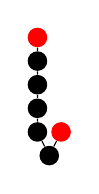
\begin{tikzpicture}[scale=.2]
\node[circle, scale=0.75, fill] (tid0) at (1.5,1.5){};
\node[circle, scale=0.75, fill] (tid1) at (0.75,3){};
\node[circle, scale=0.75, fill] (tid3) at (0.75,4.5){};
\node[circle, scale=0.75, fill] (tid4) at (0.75,6){};
\node[circle, scale=0.75, fill] (tid5) at (0.75,7.5){};
\node[circle, scale=0.75, fill, red] (tid6) at (0.75,9){};
\draw[](tid5) -- (tid6);
\draw[](tid4) -- (tid5);
\draw[](tid3) -- (tid4);
\draw[](tid1) -- (tid3);
\node[circle, scale=0.75, fill, red] (tid2) at (2.25,3){};
\draw[](tid0) -- (tid1);
\draw[](tid0) -- (tid2);
\end{tikzpicture}
\nodepart{two}
\footnotesize{6.03125}
\nodepart{three}
\footnotesize{$50\:50$}
};
\node[draw opacity=0, fill opacity=0, anchor=south west] (dummyL) at (-33, -75){};
\node[draw=black, rectangle split, anchor=south west, rectangle split parts=3] (sn0x8676118) at ([xshift=2cm]sn0x8675ff0.south east){
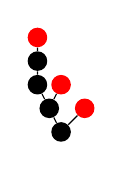
\begin{tikzpicture}[scale=.2]
\node[circle, scale=0.75, fill] (tid0) at (2.25,1.5){};
\node[circle, scale=0.75, fill] (tid1) at (1.5,3){};
\node[circle, scale=0.75, fill] (tid3) at (0.75,4.5){};
\node[circle, scale=0.75, fill] (tid5) at (0.75,6){};
\node[circle, scale=0.75, fill, red] (tid6) at (0.75,7.5){};
\draw[](tid5) -- (tid6);
\draw[](tid3) -- (tid5);
\node[circle, scale=0.75, fill, red] (tid4) at (2.25,4.5){};
\draw[](tid1) -- (tid3);
\draw[](tid1) -- (tid4);
\node[circle, scale=0.75, fill, red] (tid2) at (3.75,3){};
\draw[](tid0) -- (tid1);
\draw[](tid0) -- (tid2);
\end{tikzpicture}
\nodepart{two}
\footnotesize{5.17824}
\nodepart{three}
\footnotesize{$33\:33\:33$}
};
\node[draw opacity=0, fill opacity=0, anchor=south west] (dummyL) at (-33, -75){};
\node[draw=black, rectangle split, anchor=south west, rectangle split parts=3] (sn0x8676560) at ([xshift=2cm]sn0x8676118.south east){
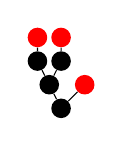
\begin{tikzpicture}[scale=.2]
\node[circle, scale=0.75, fill] (tid0) at (2.25,1.5){};
\node[circle, scale=0.75, fill] (tid1) at (1.5,3){};
\node[circle, scale=0.75, fill] (tid3) at (0.75,4.5){};
\node[circle, scale=0.75, fill, red] (tid5) at (0.75,6){};
\draw[](tid3) -- (tid5);
\node[circle, scale=0.75, fill] (tid4) at (2.25,4.5){};
\node[circle, scale=0.75, fill, red] (tid6) at (2.25,6){};
\draw[](tid4) -- (tid6);
\draw[](tid1) -- (tid3);
\draw[](tid1) -- (tid4);
\node[circle, scale=0.75, fill, red] (tid2) at (3.75,3){};
\draw[](tid0) -- (tid1);
\draw[](tid0) -- (tid2);
\end{tikzpicture}
\nodepart{two}
\footnotesize{4.81482}
\nodepart{three}
\footnotesize{$33\:67$}
};
\node[draw opacity=0, fill opacity=0, anchor=south west] (dummyL) at (-33, -75){};
\node[draw=black, rectangle split, anchor=south west, rectangle split parts=3] (sn0x8676eb0) at ([xshift=2cm]sn0x8676560.south east){
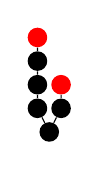
\begin{tikzpicture}[scale=.2]
\node[circle, scale=0.75, fill] (tid0) at (1.5,1.5){};
\node[circle, scale=0.75, fill] (tid1) at (0.75,3){};
\node[circle, scale=0.75, fill] (tid3) at (0.75,4.5){};
\node[circle, scale=0.75, fill] (tid5) at (0.75,6){};
\node[circle, scale=0.75, fill, red] (tid6) at (0.75,7.5){};
\draw[](tid5) -- (tid6);
\draw[](tid3) -- (tid5);
\draw[](tid1) -- (tid3);
\node[circle, scale=0.75, fill] (tid2) at (2.25,3){};
\node[circle, scale=0.75, fill, red] (tid4) at (2.25,4.5){};
\draw[](tid2) -- (tid4);
\draw[](tid0) -- (tid1);
\draw[](tid0) -- (tid2);
\end{tikzpicture}
\nodepart{two}
\footnotesize{5.25}
\nodepart{three}
\footnotesize{$50\:50$}
};
\node[draw opacity=0, fill opacity=0, anchor=south west] (dummyL) at (-33, -75){};
\node[draw=black, rectangle split, anchor=south west, rectangle split parts=3] (sn0x8677eb0) at ([xshift=2cm]sn0x8676eb0.south east){
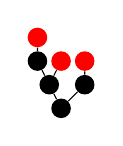
\begin{tikzpicture}[scale=.2]
\node[circle, scale=0.75, fill] (tid0) at (2.25,1.5){};
\node[circle, scale=0.75, fill] (tid1) at (1.5,3){};
\node[circle, scale=0.75, fill] (tid3) at (0.75,4.5){};
\node[circle, scale=0.75, fill, red] (tid6) at (0.75,6){};
\draw[](tid3) -- (tid6);
\node[circle, scale=0.75, fill, red] (tid4) at (2.25,4.5){};
\draw[](tid1) -- (tid3);
\draw[](tid1) -- (tid4);
\node[circle, scale=0.75, fill] (tid2) at (3.75,3){};
\node[circle, scale=0.75, fill, red] (tid5) at (3.75,4.5){};
\draw[](tid2) -- (tid5);
\draw[](tid0) -- (tid1);
\draw[](tid0) -- (tid2);
\end{tikzpicture}
\nodepart{two}
\footnotesize{4.61343}
\nodepart{three}
\footnotesize{$33\:33\:33$}
};
\node[draw opacity=0, fill opacity=0, anchor=south west] (dummyL) at (-33, -75){};
\node[draw=black, rectangle split, anchor=south west, rectangle split parts=3] (sn0x8679e68) at ([xshift=2cm]sn0x8677eb0.south east){
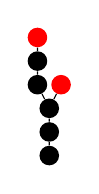
\begin{tikzpicture}[scale=.2]
\node[circle, scale=0.75, fill] (tid0) at (1.5,1.5){};
\node[circle, scale=0.75, fill] (tid1) at (1.5,3){};
\node[circle, scale=0.75, fill] (tid2) at (1.5,4.5){};
\node[circle, scale=0.75, fill] (tid3) at (0.75,6){};
\node[circle, scale=0.75, fill] (tid5) at (0.75,7.5){};
\node[circle, scale=0.75, fill, red] (tid6) at (0.75,9){};
\draw[](tid5) -- (tid6);
\draw[](tid3) -- (tid5);
\node[circle, scale=0.75, fill, red] (tid4) at (2.25,6){};
\draw[](tid2) -- (tid3);
\draw[](tid2) -- (tid4);
\draw[](tid1) -- (tid2);
\draw[](tid0) -- (tid1);
\end{tikzpicture}
\nodepart{two}
\footnotesize{6.125}
\nodepart{three}
\footnotesize{$50\:50$}
};
\node[draw opacity=0, fill opacity=0, anchor=south west] (dummyL) at (-33, -75){};
\node[draw=black, rectangle split, anchor=south west, rectangle split parts=3] (sn0x8679898) at ([xshift=2cm]sn0x8679e68.south east){
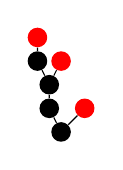
\begin{tikzpicture}[scale=.2]
\node[circle, scale=0.75, fill] (tid0) at (2.25,1.5){};
\node[circle, scale=0.75, fill] (tid1) at (1.5,3){};
\node[circle, scale=0.75, fill] (tid3) at (1.5,4.5){};
\node[circle, scale=0.75, fill] (tid4) at (0.75,6){};
\node[circle, scale=0.75, fill, red] (tid6) at (0.75,7.5){};
\draw[](tid4) -- (tid6);
\node[circle, scale=0.75, fill, red] (tid5) at (2.25,6){};
\draw[](tid3) -- (tid4);
\draw[](tid3) -- (tid5);
\draw[](tid1) -- (tid3);
\node[circle, scale=0.75, fill, red] (tid2) at (3.75,3){};
\draw[](tid0) -- (tid1);
\draw[](tid0) -- (tid2);
\end{tikzpicture}
\nodepart{two}
\footnotesize{5.29861}
\nodepart{three}
\footnotesize{$33\:33\:33$}
};
\node[draw opacity=0, fill opacity=0, anchor=south west] (dummyL) at (-33, -75){};
\node[draw=black, rectangle split, anchor=south west, rectangle split parts=3] (sn0x867a2a8) at ([xshift=2cm]sn0x8679898.south east){
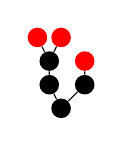
\begin{tikzpicture}[scale=.2]
\node[circle, scale=0.75, fill] (tid0) at (2.25,1.5){};
\node[circle, scale=0.75, fill] (tid1) at (1.5,3){};
\node[circle, scale=0.75, fill] (tid3) at (1.5,4.5){};
\node[circle, scale=0.75, fill, red] (tid5) at (0.75,6){};
\node[circle, scale=0.75, fill, red] (tid6) at (2.25,6){};
\draw[](tid3) -- (tid5);
\draw[](tid3) -- (tid6);
\draw[](tid1) -- (tid3);
\node[circle, scale=0.75, fill] (tid2) at (3.75,3){};
\node[circle, scale=0.75, fill, red] (tid4) at (3.75,4.5){};
\draw[](tid2) -- (tid4);
\draw[](tid0) -- (tid1);
\draw[](tid0) -- (tid2);
\end{tikzpicture}
\nodepart{two}
\footnotesize{4.81944}
\nodepart{three}
\footnotesize{$67\:33$}
};
\node[draw opacity=0, fill opacity=0, anchor=south west] (dummyL) at (-33, -75){};
\node[draw=black, rectangle split, anchor=south west, rectangle split parts=3] (sn0x867bce0) at ([xshift=2cm]sn0x867a2a8.south east){
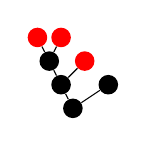
\begin{tikzpicture}[scale=.2]
\node[circle, scale=0.75, fill] (tid0) at (3,1.5){};
\node[circle, scale=0.75, fill] (tid1) at (2.25,3){};
\node[circle, scale=0.75, fill] (tid3) at (1.5,4.5){};
\node[circle, scale=0.75, fill, red] (tid5) at (0.75,6){};
\node[circle, scale=0.75, fill, red] (tid6) at (2.25,6){};
\draw[](tid3) -- (tid5);
\draw[](tid3) -- (tid6);
\node[circle, scale=0.75, fill, red] (tid4) at (3.75,4.5){};
\draw[](tid1) -- (tid3);
\draw[](tid1) -- (tid4);
\node[circle, scale=0.75, fill] (tid2) at (5.25,3){};
\draw[](tid0) -- (tid1);
\draw[](tid0) -- (tid2);
\end{tikzpicture}
\nodepart{two}
\footnotesize{4.75926}
\nodepart{three}
\footnotesize{$67\:33$}
};
\node[draw opacity=0, fill opacity=0, anchor=south west] (dummyL) at (-27, -90){};
\node[draw=black, rectangle split, anchor=south west, rectangle split parts=3] (sn0x8674d78) at ([xshift=2cm]dummyL){
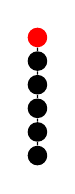
\begin{tikzpicture}[scale=.2]
\node[circle, scale=0.75, fill] (tid0) at (0.75,1.5){};
\node[circle, scale=0.75, fill] (tid1) at (0.75,3){};
\node[circle, scale=0.75, fill] (tid2) at (0.75,4.5){};
\node[circle, scale=0.75, fill] (tid3) at (0.75,6){};
\node[circle, scale=0.75, fill] (tid4) at (0.75,7.5){};
\node[circle, scale=0.75, fill, red] (tid5) at (0.75,9){};
\draw[](tid4) -- (tid5);
\draw[](tid3) -- (tid4);
\draw[](tid2) -- (tid3);
\draw[](tid1) -- (tid2);
\draw[](tid0) -- (tid1);
\end{tikzpicture}
\nodepart{two}
\footnotesize{6}
\nodepart{three}
\footnotesize{$1$}
};
\node[draw opacity=0, fill opacity=0, anchor=south west] (dummyL) at (-27, -90){};
\node[draw=black, rectangle split, anchor=south west, rectangle split parts=3] (sn0x86753c0) at ([xshift=2cm]sn0x8674d78.south east){
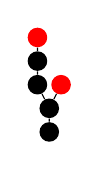
\begin{tikzpicture}[scale=.2]
\node[circle, scale=0.75, fill] (tid0) at (1.5,1.5){};
\node[circle, scale=0.75, fill] (tid1) at (1.5,3){};
\node[circle, scale=0.75, fill] (tid2) at (0.75,4.5){};
\node[circle, scale=0.75, fill] (tid4) at (0.75,6){};
\node[circle, scale=0.75, fill, red] (tid5) at (0.75,7.5){};
\draw[](tid4) -- (tid5);
\draw[](tid2) -- (tid4);
\node[circle, scale=0.75, fill, red] (tid3) at (2.25,4.5){};
\draw[](tid1) -- (tid2);
\draw[](tid1) -- (tid3);
\draw[](tid0) -- (tid1);
\end{tikzpicture}
\nodepart{two}
\footnotesize{5.125}
\nodepart{three}
\footnotesize{$50\:50$}
};
\node[draw opacity=0, fill opacity=0, anchor=south west] (dummyL) at (-27, -90){};
\node[draw=black, rectangle split, anchor=south west, rectangle split parts=3] (sn0x86762e8) at ([xshift=2cm]sn0x86753c0.south east){
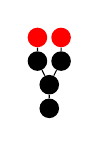
\begin{tikzpicture}[scale=.2]
\node[circle, scale=0.75, fill] (tid0) at (1.5,1.5){};
\node[circle, scale=0.75, fill] (tid1) at (1.5,3){};
\node[circle, scale=0.75, fill] (tid2) at (0.75,4.5){};
\node[circle, scale=0.75, fill, red] (tid4) at (0.75,6){};
\draw[](tid2) -- (tid4);
\node[circle, scale=0.75, fill] (tid3) at (2.25,4.5){};
\node[circle, scale=0.75, fill, red] (tid5) at (2.25,6){};
\draw[](tid3) -- (tid5);
\draw[](tid1) -- (tid2);
\draw[](tid1) -- (tid3);
\draw[](tid0) -- (tid1);
\end{tikzpicture}
\nodepart{two}
\footnotesize{4.75}
\nodepart{three}
\footnotesize{$1$}
};
\node[draw opacity=0, fill opacity=0, anchor=south west] (dummyL) at (-27, -90){};
\node[draw=black, rectangle split, anchor=south west, rectangle split parts=3] (sn0x8675a18) at ([xshift=2cm]sn0x86762e8.south east){
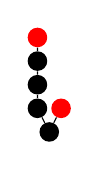
\begin{tikzpicture}[scale=.2]
\node[circle, scale=0.75, fill] (tid0) at (1.5,1.5){};
\node[circle, scale=0.75, fill] (tid1) at (0.75,3){};
\node[circle, scale=0.75, fill] (tid3) at (0.75,4.5){};
\node[circle, scale=0.75, fill] (tid4) at (0.75,6){};
\node[circle, scale=0.75, fill, red] (tid5) at (0.75,7.5){};
\draw[](tid4) -- (tid5);
\draw[](tid3) -- (tid4);
\draw[](tid1) -- (tid3);
\node[circle, scale=0.75, fill, red] (tid2) at (2.25,3){};
\draw[](tid0) -- (tid1);
\draw[](tid0) -- (tid2);
\end{tikzpicture}
\nodepart{two}
\footnotesize{5.0625}
\nodepart{three}
\footnotesize{$50\:50$}
};
\node[draw opacity=0, fill opacity=0, anchor=south west] (dummyL) at (-27, -90){};
\node[draw=black, rectangle split, anchor=south west, rectangle split parts=3] (sn0x86773c8) at ([xshift=2cm]sn0x8675a18.south east){
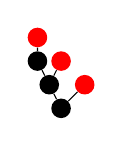
\begin{tikzpicture}[scale=.2]
\node[circle, scale=0.75, fill] (tid0) at (2.25,1.5){};
\node[circle, scale=0.75, fill] (tid1) at (1.5,3){};
\node[circle, scale=0.75, fill] (tid3) at (0.75,4.5){};
\node[circle, scale=0.75, fill, red] (tid5) at (0.75,6){};
\draw[](tid3) -- (tid5);
\node[circle, scale=0.75, fill, red] (tid4) at (2.25,4.5){};
\draw[](tid1) -- (tid3);
\draw[](tid1) -- (tid4);
\node[circle, scale=0.75, fill, red] (tid2) at (3.75,3){};
\draw[](tid0) -- (tid1);
\draw[](tid0) -- (tid2);
\end{tikzpicture}
\nodepart{two}
\footnotesize{4.34722}
\nodepart{three}
\footnotesize{$33\:33\:33$}
};
\node[draw opacity=0, fill opacity=0, anchor=south west] (dummyL) at (-27, -90){};
\node[draw=black, rectangle split, anchor=south west, rectangle split parts=3] (sn0x8677c38) at ([xshift=2cm]sn0x86773c8.south east){
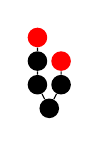
\begin{tikzpicture}[scale=.2]
\node[circle, scale=0.75, fill] (tid0) at (1.5,1.5){};
\node[circle, scale=0.75, fill] (tid1) at (0.75,3){};
\node[circle, scale=0.75, fill] (tid3) at (0.75,4.5){};
\node[circle, scale=0.75, fill, red] (tid5) at (0.75,6){};
\draw[](tid3) -- (tid5);
\draw[](tid1) -- (tid3);
\node[circle, scale=0.75, fill] (tid2) at (2.25,3){};
\node[circle, scale=0.75, fill, red] (tid4) at (2.25,4.5){};
\draw[](tid2) -- (tid4);
\draw[](tid0) -- (tid1);
\draw[](tid0) -- (tid2);
\end{tikzpicture}
\nodepart{two}
\footnotesize{4.4375}
\nodepart{three}
\footnotesize{$50\:50$}
};
\node[draw opacity=0, fill opacity=0, anchor=south west] (dummyL) at (-27, -90){};
\node[draw=black, rectangle split, anchor=south west, rectangle split parts=3] (sn0x8677fd8) at ([xshift=2cm]sn0x8677c38.south east){
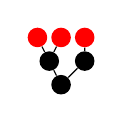
\begin{tikzpicture}[scale=.2]
\node[circle, scale=0.75, fill] (tid0) at (2.25,1.5){};
\node[circle, scale=0.75, fill] (tid1) at (1.5,3){};
\node[circle, scale=0.75, fill, red] (tid3) at (0.75,4.5){};
\node[circle, scale=0.75, fill, red] (tid4) at (2.25,4.5){};
\draw[](tid1) -- (tid3);
\draw[](tid1) -- (tid4);
\node[circle, scale=0.75, fill] (tid2) at (3.75,3){};
\node[circle, scale=0.75, fill, red] (tid5) at (3.75,4.5){};
\draw[](tid2) -- (tid5);
\draw[](tid0) -- (tid1);
\draw[](tid0) -- (tid2);
\end{tikzpicture}
\nodepart{two}
\footnotesize{4.05556}
\nodepart{three}
\footnotesize{$33\:67$}
};
\node[draw opacity=0, fill opacity=0, anchor=south west] (dummyL) at (-27, -90){};
\node[draw=black, rectangle split, anchor=south west, rectangle split parts=3] (sn0x867a4b0) at ([xshift=2cm]sn0x8677fd8.south east){
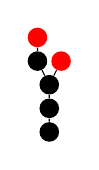
\begin{tikzpicture}[scale=.2]
\node[circle, scale=0.75, fill] (tid0) at (1.5,1.5){};
\node[circle, scale=0.75, fill] (tid1) at (1.5,3){};
\node[circle, scale=0.75, fill] (tid2) at (1.5,4.5){};
\node[circle, scale=0.75, fill] (tid3) at (0.75,6){};
\node[circle, scale=0.75, fill, red] (tid5) at (0.75,7.5){};
\draw[](tid3) -- (tid5);
\node[circle, scale=0.75, fill, red] (tid4) at (2.25,6){};
\draw[](tid2) -- (tid3);
\draw[](tid2) -- (tid4);
\draw[](tid1) -- (tid2);
\draw[](tid0) -- (tid1);
\end{tikzpicture}
\nodepart{two}
\footnotesize{5.25}
\nodepart{three}
\footnotesize{$50\:50$}
};
\node[draw opacity=0, fill opacity=0, anchor=south west] (dummyL) at (-27, -90){};
\node[draw=black, rectangle split, anchor=south west, rectangle split parts=3] (sn0x867a830) at ([xshift=2cm]sn0x867a4b0.south east){
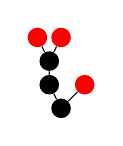
\begin{tikzpicture}[scale=.2]
\node[circle, scale=0.75, fill] (tid0) at (2.25,1.5){};
\node[circle, scale=0.75, fill] (tid1) at (1.5,3){};
\node[circle, scale=0.75, fill] (tid3) at (1.5,4.5){};
\node[circle, scale=0.75, fill, red] (tid4) at (0.75,6){};
\node[circle, scale=0.75, fill, red] (tid5) at (2.25,6){};
\draw[](tid3) -- (tid4);
\draw[](tid3) -- (tid5);
\draw[](tid1) -- (tid3);
\node[circle, scale=0.75, fill, red] (tid2) at (3.75,3){};
\draw[](tid0) -- (tid1);
\draw[](tid0) -- (tid2);
\end{tikzpicture}
\nodepart{two}
\footnotesize{4.58333}
\nodepart{three}
\footnotesize{$67\:33$}
};
\node[draw opacity=0, fill opacity=0, anchor=south west] (dummyL) at (-18, -105){};
\node[draw=black, rectangle split, anchor=south west, rectangle split parts=3] (sn0x8675068) at ([xshift=2cm]dummyL){
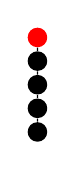
\begin{tikzpicture}[scale=.2]
\node[circle, scale=0.75, fill] (tid0) at (0.75,1.5){};
\node[circle, scale=0.75, fill] (tid1) at (0.75,3){};
\node[circle, scale=0.75, fill] (tid2) at (0.75,4.5){};
\node[circle, scale=0.75, fill] (tid3) at (0.75,6){};
\node[circle, scale=0.75, fill, red] (tid4) at (0.75,7.5){};
\draw[](tid3) -- (tid4);
\draw[](tid2) -- (tid3);
\draw[](tid1) -- (tid2);
\draw[](tid0) -- (tid1);
\end{tikzpicture}
\nodepart{two}
\footnotesize{5}
\nodepart{three}
\footnotesize{$1$}
};
\node[draw opacity=0, fill opacity=0, anchor=south west] (dummyL) at (-18, -105){};
\node[draw=black, rectangle split, anchor=south west, rectangle split parts=3] (sn0x8675718) at ([xshift=2cm]sn0x8675068.south east){
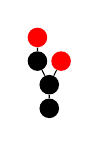
\begin{tikzpicture}[scale=.2]
\node[circle, scale=0.75, fill] (tid0) at (1.5,1.5){};
\node[circle, scale=0.75, fill] (tid1) at (1.5,3){};
\node[circle, scale=0.75, fill] (tid2) at (0.75,4.5){};
\node[circle, scale=0.75, fill, red] (tid4) at (0.75,6){};
\draw[](tid2) -- (tid4);
\node[circle, scale=0.75, fill, red] (tid3) at (2.25,4.5){};
\draw[](tid1) -- (tid2);
\draw[](tid1) -- (tid3);
\draw[](tid0) -- (tid1);
\end{tikzpicture}
\nodepart{two}
\footnotesize{4.25}
\nodepart{three}
\footnotesize{$50\:50$}
};
\node[draw opacity=0, fill opacity=0, anchor=south west] (dummyL) at (-18, -105){};
\node[draw=black, rectangle split, anchor=south west, rectangle split parts=3] (sn0x8676918) at ([xshift=2cm]sn0x8675718.south east){
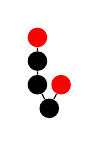
\begin{tikzpicture}[scale=.2]
\node[circle, scale=0.75, fill] (tid0) at (1.5,1.5){};
\node[circle, scale=0.75, fill] (tid1) at (0.75,3){};
\node[circle, scale=0.75, fill] (tid3) at (0.75,4.5){};
\node[circle, scale=0.75, fill, red] (tid4) at (0.75,6){};
\draw[](tid3) -- (tid4);
\draw[](tid1) -- (tid3);
\node[circle, scale=0.75, fill, red] (tid2) at (2.25,3){};
\draw[](tid0) -- (tid1);
\draw[](tid0) -- (tid2);
\end{tikzpicture}
\nodepart{two}
\footnotesize{4.125}
\nodepart{three}
\footnotesize{$50\:50$}
};
\node[draw opacity=0, fill opacity=0, anchor=south west] (dummyL) at (-18, -105){};
\node[draw=black, rectangle split, anchor=south west, rectangle split parts=3] (sn0x8677118) at ([xshift=2cm]sn0x8676918.south east){
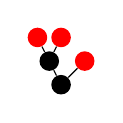
\begin{tikzpicture}[scale=.2]
\node[circle, scale=0.75, fill] (tid0) at (2.25,1.5){};
\node[circle, scale=0.75, fill] (tid1) at (1.5,3){};
\node[circle, scale=0.75, fill, red] (tid3) at (0.75,4.5){};
\node[circle, scale=0.75, fill, red] (tid4) at (2.25,4.5){};
\draw[](tid1) -- (tid3);
\draw[](tid1) -- (tid4);
\node[circle, scale=0.75, fill, red] (tid2) at (3.75,3){};
\draw[](tid0) -- (tid1);
\draw[](tid0) -- (tid2);
\end{tikzpicture}
\nodepart{two}
\footnotesize{3.66667}
\nodepart{three}
\footnotesize{$33\:67$}
};
\node[draw opacity=0, fill opacity=0, anchor=south west] (dummyL) at (-18, -105){};
\node[draw=black, rectangle split, anchor=south west, rectangle split parts=3] (sn0x8677d38) at ([xshift=2cm]sn0x8677118.south east){
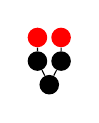
\begin{tikzpicture}[scale=.2]
\node[circle, scale=0.75, fill] (tid0) at (1.5,1.5){};
\node[circle, scale=0.75, fill] (tid1) at (0.75,3){};
\node[circle, scale=0.75, fill, red] (tid3) at (0.75,4.5){};
\draw[](tid1) -- (tid3);
\node[circle, scale=0.75, fill] (tid2) at (2.25,3){};
\node[circle, scale=0.75, fill, red] (tid4) at (2.25,4.5){};
\draw[](tid2) -- (tid4);
\draw[](tid0) -- (tid1);
\draw[](tid0) -- (tid2);
\end{tikzpicture}
\nodepart{two}
\footnotesize{3.75}
\nodepart{three}
\footnotesize{$1$}
};
\node[draw opacity=0, fill opacity=0, anchor=south west] (dummyL) at (-18, -105){};
\node[draw=black, rectangle split, anchor=south west, rectangle split parts=3] (sn0x867a3d0) at ([xshift=2cm]sn0x8677d38.south east){
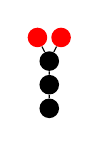
\begin{tikzpicture}[scale=.2]
\node[circle, scale=0.75, fill] (tid0) at (1.5,1.5){};
\node[circle, scale=0.75, fill] (tid1) at (1.5,3){};
\node[circle, scale=0.75, fill] (tid2) at (1.5,4.5){};
\node[circle, scale=0.75, fill, red] (tid3) at (0.75,6){};
\node[circle, scale=0.75, fill, red] (tid4) at (2.25,6){};
\draw[](tid2) -- (tid3);
\draw[](tid2) -- (tid4);
\draw[](tid1) -- (tid2);
\draw[](tid0) -- (tid1);
\end{tikzpicture}
\nodepart{two}
\footnotesize{4.5}
\nodepart{three}
\footnotesize{$1$}
};
\node[draw opacity=0, fill opacity=0, anchor=south west] (dummyL) at (-9, -120){};
\node[draw=black, rectangle split, anchor=south west, rectangle split parts=3] (sn0x86751e0) at ([xshift=2cm]dummyL){
\begin{tikzpicture}[scale=.2]
\node[circle, scale=0.75, fill] (tid0) at (0.75,1.5){};
\node[circle, scale=0.75, fill] (tid1) at (0.75,3){};
\node[circle, scale=0.75, fill] (tid2) at (0.75,4.5){};
\node[circle, scale=0.75, fill, red] (tid3) at (0.75,6){};
\draw[](tid2) -- (tid3);
\draw[](tid1) -- (tid2);
\draw[](tid0) -- (tid1);
\end{tikzpicture}
\nodepart{two}
\footnotesize{4}
\nodepart{three}
\footnotesize{$1$}
};
\node[draw opacity=0, fill opacity=0, anchor=south west] (dummyL) at (-9, -120){};
\node[draw=black, rectangle split, anchor=south west, rectangle split parts=3] (sn0x8675688) at ([xshift=2cm]sn0x86751e0.south east){
\begin{tikzpicture}[scale=.2]
\node[circle, scale=0.75, fill] (tid0) at (1.5,1.5){};
\node[circle, scale=0.75, fill] (tid1) at (1.5,3){};
\node[circle, scale=0.75, fill, red] (tid2) at (0.75,4.5){};
\node[circle, scale=0.75, fill, red] (tid3) at (2.25,4.5){};
\draw[](tid1) -- (tid2);
\draw[](tid1) -- (tid3);
\draw[](tid0) -- (tid1);
\end{tikzpicture}
\nodepart{two}
\footnotesize{3.5}
\nodepart{three}
\footnotesize{$1$}
};
\node[draw opacity=0, fill opacity=0, anchor=south west] (dummyL) at (-9, -120){};
\node[draw=black, rectangle split, anchor=south west, rectangle split parts=3] (sn0x8676e20) at ([xshift=2cm]sn0x8675688.south east){
\begin{tikzpicture}[scale=.2]
\node[circle, scale=0.75, fill] (tid0) at (1.5,1.5){};
\node[circle, scale=0.75, fill] (tid1) at (0.75,3){};
\node[circle, scale=0.75, fill, red] (tid3) at (0.75,4.5){};
\draw[](tid1) -- (tid3);
\node[circle, scale=0.75, fill, red] (tid2) at (2.25,3){};
\draw[](tid0) -- (tid1);
\draw[](tid0) -- (tid2);
\end{tikzpicture}
\nodepart{two}
\footnotesize{3.25}
\nodepart{three}
\footnotesize{$50\:50$}
};
\node[draw opacity=0, fill opacity=0, anchor=south west] (dummyL) at (-6, -135){};
\node[draw=black, rectangle split, anchor=south west, rectangle split parts=3] (sn0x8675618) at ([xshift=2cm]dummyL){
\begin{tikzpicture}[scale=.2]
\node[circle, scale=0.75, fill] (tid0) at (0.75,1.5){};
\node[circle, scale=0.75, fill] (tid1) at (0.75,3){};
\node[circle, scale=0.75, fill, red] (tid2) at (0.75,4.5){};
\draw[](tid1) -- (tid2);
\draw[](tid0) -- (tid1);
\end{tikzpicture}
\nodepart{two}
\footnotesize{3}
\nodepart{three}
\footnotesize{$1$}
};
\node[draw opacity=0, fill opacity=0, anchor=south west] (dummyL) at (-6, -135){};
\node[draw=black, rectangle split, anchor=south west, rectangle split parts=3] (sn0x8676c98) at ([xshift=2cm]sn0x8675618.south east){
\begin{tikzpicture}[scale=.2]
\node[circle, scale=0.75, fill] (tid0) at (1.5,1.5){};
\node[circle, scale=0.75, fill, red] (tid1) at (0.75,3){};
\node[circle, scale=0.75, fill, red] (tid2) at (2.25,3){};
\draw[](tid0) -- (tid1);
\draw[](tid0) -- (tid2);
\end{tikzpicture}
\nodepart{two}
\footnotesize{2.5}
\nodepart{three}
\footnotesize{$1$}
};
\node[draw opacity=0, fill opacity=0, anchor=south west] (dummyL) at (-3, -150){};
\node[draw=black, rectangle split, anchor=south west, rectangle split parts=3] (sn0x86742c8) at ([xshift=2cm]dummyL){
\begin{tikzpicture}[scale=.2]
\node[circle, scale=0.75, fill] (tid0) at (0.75,1.5){};
\node[circle, scale=0.75, fill, red] (tid1) at (0.75,3){};
\draw[](tid0) -- (tid1);
\end{tikzpicture}
\nodepart{two}
\footnotesize{2}
\nodepart{three}
\footnotesize{$1$}
};
\node[draw opacity=0, fill opacity=0, anchor=south west] (dummyL) at (-3, -165){};
\node[draw=black, rectangle split, anchor=south west, rectangle split parts=3] (sn0x8674358) at ([xshift=2cm]dummyL){
\begin{tikzpicture}[scale=.2]
\node[circle, scale=0.75, fill, red] (tid0) at (0.75,1.5){};
\end{tikzpicture}
\nodepart{two}
\footnotesize{1}
\nodepart{three}
\footnotesize{$$}
};
\draw (sn0x8671148.south) -- (sn0x8673440.north);
\draw (sn0x8671148.south) -- (sn0x8672868.north);
\draw (sn0x8671148.south) -- (sn0x86715f8.north);
\draw (sn0x8671148.south) -- (sn0x8671730.north);
\draw (sn0x8673440.south) -- (sn0x8674070.north);
\draw (sn0x8673440.south) -- (sn0x8670960.north);
\draw (sn0x8673440.south) -- (sn0x8671f38.north);
\draw (sn0x8672868.south) -- (sn0x8679150.north);
\draw (sn0x8672868.south) -- (sn0x8670960.north);
\draw (sn0x8672868.south) -- (sn0x8678838.north);
\draw (sn0x86715f8.south) -- (sn0x867b748.north);
\draw (sn0x86715f8.south) -- (sn0x8670960.north);
\draw (sn0x86715f8.south) -- (sn0x867b6e8.north);
\draw (sn0x8671730.south) -- (sn0x8671f38.north);
\draw (sn0x8671730.south) -- (sn0x8678838.north);
\draw (sn0x8671730.south) -- (sn0x867b6e8.north);
\draw (sn0x8671730.south) -- (sn0x867c970.north);
\draw (sn0x8674070.south) -- (sn0x86717a8.north);
\draw (sn0x8674070.south) -- (sn0x8674958.north);
\draw (sn0x8674070.south) -- (sn0x8674cb0.north);
\draw (sn0x8670960.south) -- (sn0x8677a00.north);
\draw (sn0x8670960.south) -- (sn0x8674958.north);
\draw (sn0x8670960.south) -- (sn0x8677b20.north);
\draw (sn0x8671f38.south) -- (sn0x8674cb0.north);
\draw (sn0x8671f38.south) -- (sn0x8677b20.north);
\draw (sn0x8671f38.south) -- (sn0x86791a8.north);
\draw (sn0x8679150.south) -- (sn0x8679ac0.north);
\draw (sn0x8679150.south) -- (sn0x8677a00.north);
\draw (sn0x8679150.south) -- (sn0x8679030.north);
\draw (sn0x8678838.south) -- (sn0x8679030.north);
\draw (sn0x8678838.south) -- (sn0x8677b20.north);
\draw (sn0x8678838.south) -- (sn0x867b2e0.north);
\draw (sn0x867b748.south) -- (sn0x8679ac0.north);
\draw (sn0x867b748.south) -- (sn0x8674958.north);
\draw (sn0x867b748.south) -- (sn0x867a9c8.north);
\draw (sn0x867b6e8.south) -- (sn0x867a9c8.north);
\draw (sn0x867b6e8.south) -- (sn0x8677b20.north);
\draw (sn0x867b6e8.south) -- (sn0x867b7c8.north);
\draw (sn0x867c970.south) -- (sn0x86791a8.north);
\draw (sn0x867c970.south) -- (sn0x867b2e0.north);
\draw (sn0x867c970.south) -- (sn0x867b7c8.north);
\draw (sn0x86717a8.south) -- (sn0x8671678.north);
\draw (sn0x86717a8.south) -- (sn0x8674888.north);
\draw (sn0x8674958.south) -- (sn0x8671678.north);
\draw (sn0x8674958.south) -- (sn0x8675ff0.north);
\draw (sn0x8674958.south) -- (sn0x8676118.north);
\draw (sn0x8674cb0.south) -- (sn0x8674888.north);
\draw (sn0x8674cb0.south) -- (sn0x8676118.north);
\draw (sn0x8674cb0.south) -- (sn0x8676560.north);
\draw (sn0x8677a00.south) -- (sn0x8675ff0.north);
\draw (sn0x8677a00.south) -- (sn0x8676eb0.north);
\draw (sn0x8677b20.south) -- (sn0x8676eb0.north);
\draw (sn0x8677b20.south) -- (sn0x8676118.north);
\draw (sn0x8677b20.south) -- (sn0x8677eb0.north);
\draw (sn0x86791a8.south) -- (sn0x8676560.north);
\draw (sn0x86791a8.south) -- (sn0x8677eb0.north);
\draw (sn0x8679ac0.south) -- (sn0x8679e68.north);
\draw (sn0x8679ac0.south) -- (sn0x8675ff0.north);
\draw (sn0x8679ac0.south) -- (sn0x8679898.north);
\draw (sn0x8679030.south) -- (sn0x8679898.north);
\draw (sn0x8679030.south) -- (sn0x8676eb0.north);
\draw (sn0x8679030.south) -- (sn0x867a2a8.north);
\draw (sn0x867b2e0.south) -- (sn0x867a2a8.north);
\draw (sn0x867b2e0.south) -- (sn0x8677eb0.north);
\draw (sn0x867a9c8.south) -- (sn0x8679898.north);
\draw (sn0x867a9c8.south) -- (sn0x8676118.north);
\draw (sn0x867a9c8.south) -- (sn0x867bce0.north);
\draw (sn0x867b7c8.south) -- (sn0x867bce0.north);
\draw (sn0x867b7c8.south) -- (sn0x8677eb0.north);
\draw (sn0x8671678.south) -- (sn0x8674d78.north);
\draw (sn0x8671678.south) -- (sn0x86753c0.north);
\draw (sn0x8674888.south) -- (sn0x86753c0.north);
\draw (sn0x8674888.south) -- (sn0x86762e8.north);
\draw (sn0x8675ff0.south) -- (sn0x8674d78.north);
\draw (sn0x8675ff0.south) -- (sn0x8675a18.north);
\draw (sn0x8676118.south) -- (sn0x86753c0.north);
\draw (sn0x8676118.south) -- (sn0x8675a18.north);
\draw (sn0x8676118.south) -- (sn0x86773c8.north);
\draw (sn0x8676560.south) -- (sn0x86762e8.north);
\draw (sn0x8676560.south) -- (sn0x86773c8.north);
\draw (sn0x8676eb0.south) -- (sn0x8675a18.north);
\draw (sn0x8676eb0.south) -- (sn0x8677c38.north);
\draw (sn0x8677eb0.south) -- (sn0x8677c38.north);
\draw (sn0x8677eb0.south) -- (sn0x86773c8.north);
\draw (sn0x8677eb0.south) -- (sn0x8677fd8.north);
\draw (sn0x8679e68.south) -- (sn0x8674d78.north);
\draw (sn0x8679e68.south) -- (sn0x867a4b0.north);
\draw (sn0x8679898.south) -- (sn0x867a4b0.north);
\draw (sn0x8679898.south) -- (sn0x8675a18.north);
\draw (sn0x8679898.south) -- (sn0x867a830.north);
\draw (sn0x867a2a8.south) -- (sn0x867a830.north);
\draw (sn0x867a2a8.south) -- (sn0x8677c38.north);
\draw (sn0x867bce0.south) -- (sn0x867a830.north);
\draw (sn0x867bce0.south) -- (sn0x86773c8.north);
\draw (sn0x8674d78.south) -- (sn0x8675068.north);
\draw (sn0x86753c0.south) -- (sn0x8675068.north);
\draw (sn0x86753c0.south) -- (sn0x8675718.north);
\draw (sn0x86762e8.south) -- (sn0x8675718.north);
\draw (sn0x8675a18.south) -- (sn0x8675068.north);
\draw (sn0x8675a18.south) -- (sn0x8676918.north);
\draw (sn0x86773c8.south) -- (sn0x8675718.north);
\draw (sn0x86773c8.south) -- (sn0x8676918.north);
\draw (sn0x86773c8.south) -- (sn0x8677118.north);
\draw (sn0x8677c38.south) -- (sn0x8676918.north);
\draw (sn0x8677c38.south) -- (sn0x8677d38.north);
\draw (sn0x8677fd8.south) -- (sn0x8677d38.north);
\draw (sn0x8677fd8.south) -- (sn0x8677118.north);
\draw (sn0x867a4b0.south) -- (sn0x8675068.north);
\draw (sn0x867a4b0.south) -- (sn0x867a3d0.north);
\draw (sn0x867a830.south) -- (sn0x867a3d0.north);
\draw (sn0x867a830.south) -- (sn0x8676918.north);
\draw (sn0x8675068.south) -- (sn0x86751e0.north);
\draw (sn0x8675718.south) -- (sn0x86751e0.north);
\draw (sn0x8675718.south) -- (sn0x8675688.north);
\draw (sn0x8676918.south) -- (sn0x86751e0.north);
\draw (sn0x8676918.south) -- (sn0x8676e20.north);
\draw (sn0x8677118.south) -- (sn0x8675688.north);
\draw (sn0x8677118.south) -- (sn0x8676e20.north);
\draw (sn0x8677d38.south) -- (sn0x8676e20.north);
\draw (sn0x867a3d0.south) -- (sn0x86751e0.north);
\draw (sn0x86751e0.south) -- (sn0x8675618.north);
\draw (sn0x8675688.south) -- (sn0x8675618.north);
\draw (sn0x8676e20.south) -- (sn0x8675618.north);
\draw (sn0x8676e20.south) -- (sn0x8676c98.north);
\draw (sn0x8675618.south) -- (sn0x86742c8.north);
\draw (sn0x8676c98.south) -- (sn0x86742c8.north);
\draw (sn0x86742c8.south) -- (sn0x8674358.north);
\end{tikzpicture}

%%% Local Variables:
%%% TeX-master: "thesis/thesis.tex"
%%% End: 
